\clearpage
\section{维护 Resharding 脚本的更多背景}
\label{sec:reshard_scripts}

\begin{figure}[!t]
  \centering
  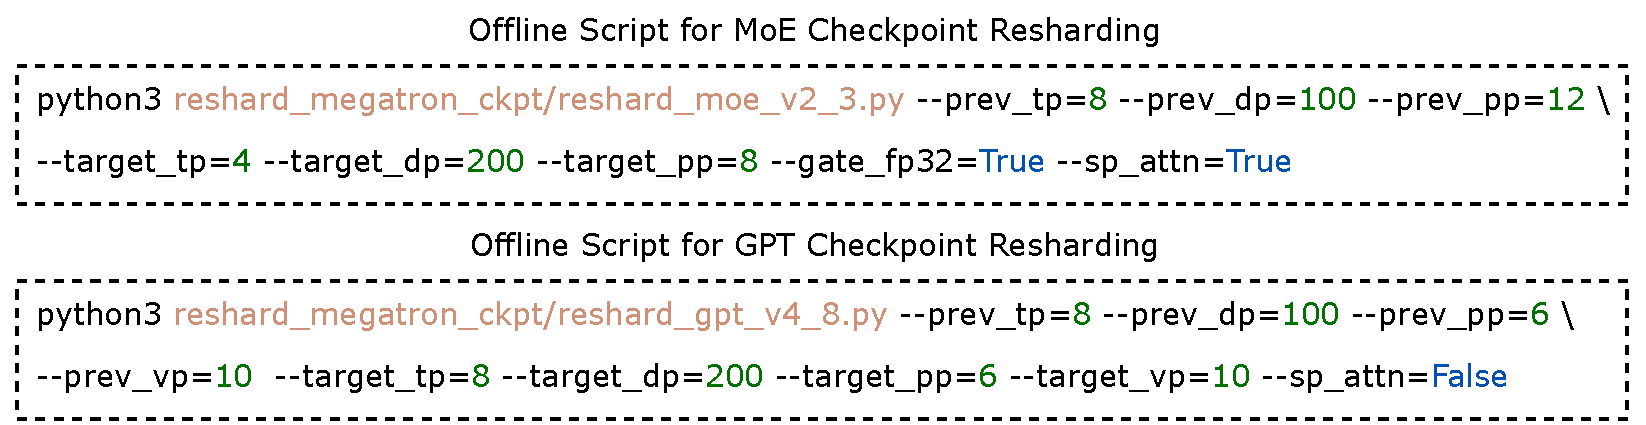
\includegraphics[width=\linewidth]{figures/scripts_example.pdf}
  \caption{
  离线 resharding 脚本运行示例。
  }
  \label{fig:script_example}
\end{figure}

图~\ref{fig:script_example} 展示了使用定制脚本进行离线 resharding 的示例。
定制离线脚本缺乏扩展性且开发成本高。
对于 GPU 状态 resharding，脚本必须覆盖 LFM 与其优化器的所有组件，并适配不同 parallelism 策略下各组件的差异行为。
例如，在 Tensor Parallelism（TP）下，注意力与 MLP 模块中的两个 GEMM 操作沿不同维度分片，而 LayerNorm~\cite{layernorm} 等算子则在 GPU 间复制。
当采用 3D 混合并行~\cite{megatron-lm2} 时，分布式优化器中的 TP 分片张量会先被扁平化并合并，再按指定的 Data Parallelism（DP）度进行分片。
离线脚本必须实现与模型（优化器）组件和 parallelism 组合强耦合的 resharding 逻辑。
此外，GQA~\cite{gqa} 与 MLA~\cite{deepseek} 等算法优化会改变某些算子的 tensor 布局（如注意力块中的 QKV 投影 GEMM），也需要相应的 resharding 支持。
为应对生产环境中的多种情况，我们维护了多个版本的 resharding 脚本，最大的一份甚至包含 3193 行 Python 代码。
这种复杂性带来了显著的开发与维护负担。

\section{高效的完整性保障}
\label{sec:barrier_check}

一个完整 checkpoint 由多个 worker 写入的多个文件组成，任一 worker 失败都可能导致 checkpoint 不完整。
因此，需要 barrier 机制在所有训练 worker 间实现保存/加载操作的原子性。

诸如 Megatron-LM~\cite{megatron} 的 checkpointing 模块使用 \texttt{torch.distributed} 的 \texttt{barrier} 来做完整性检查，该方式会同步所有 worker，确保保存/加载完成，但也带来训练阻塞。
我们观察到，当训练规模达到约 10,000 GPUs 时，每次 barrier 会造成约 20 秒的 stall。
为降低该开销，我们使用前述 gRPC + 树形分层通信拓扑重实现 \texttt{barrier}，并将完整性检查异步化，从而消除阻塞时间。
同时，\sys{} 的 I/O worker 内置上传/下载重试机制，并集成失败日志，记录未完成 checkpoint 任务的 worker 在保存/加载 pipeline 中的失败阶段，便于进一步诊断。

\section{平均 ETTR 计算}\label{sec:ettr_cal}
训练中的故障会引入进度损失与最近一次 checkpoint 加载开销。
假设故障在每个 checkpoint 间隔内均匀分布~\cite{gemini-sys}，最优情况是故障发生在一次端到端保存刚完成之后，最差情况是发生在保存即将完成之前。
给定每步训练时间 $T_{iter}$、checkpoint 间隔 $N$、端到端保存时间 $T_{save}$ 与加载（resharding）时间 $T_{load}$，平均浪费时间 $T_{wasted}$ 为：
\begin{equation}
    T_{wasted} = T_{save} + T_{load} + \frac{N \cdot T_{iter}}{2}
\end{equation}
因此平均 ETTR 为：
\begin{equation}
    ETTR = 1 - \frac{T_{wasted}}{T_{save} + T_{load} + N\cdot T_{iter}}
\end{equation}

表~\ref{tab:io_compare} 中的端到端 ETTR 结果为标准加载与 resharding 设置下的平均值。



\section{Checkpointing 开销分解}
\label{sec:save_breakdown}
我们将 rank 0 的端到端 checkpoint 保存时间（$\mathbf{T_{save}}$）拆解为多个阶段，并分析各部分开销。
结果如表~\ref{tab:save_breakdown} 所示，其中 $\mathbf{T_{Plan}^{First}}$ 表示首次规划成本，$\mathbf{T_{Plan}^{Cache}}$ 表示后续使用 plan 与 metadata 缓存时的开销。
其他阶段开销取多个 checkpoint 步的平均值。
我们发现，随着训练规模增大，规划的通信开销显著上升并导致明显 stall。
得益于缓存策略（Sec.~\ref{sec:opt_plan}），规划成本可转化为每次（恢复后的）训练会话的一次性支出。
此外，固定页 CPU 内存池使 D2H 阻塞几乎可以忽略；异步 engine pipeline 将序列化、共享内存 dump 与 HDFS 上传阶段重叠，从而缩短端到端时间。
负载均衡机制也提升了 DP 组内的并行上传能力，在更大规模下带来更多收益（例如，4800 GPUs 的模型状态上传速度比 2400 GPUs 快 3.03$\times$）。

\begin{table*}[!t]
\caption{rank 0 上 checkpoint 保存过程的详细开销分解。}
\label{tab:save_breakdown}
\begin{small}
\resizebox{\linewidth}{!}{
\begin{tabular}{c|cc|ccccccc}
    \toprule
    \textbf{Model and Framework} & \textbf{Source \#GPUs} & \textbf{State} & $\mathbf{T_{Plan}^{First}}$ \textbf{(s)} & $\mathbf{T_{Plan}^{Cache}}$ \textbf{(s)} & $\mathbf{T_{D2H}}$ \textbf{(s)} & $\mathbf{T_{Serialize}}$ \textbf{(s)} & $\mathbf{T_{Dump}}$ \textbf{(s)} & $\mathbf{T_{Upload}}$ \textbf{(s)}\\
    \midrule
     \multirow{2}{*}{vDiT 4B} & \multirow{2}{*}{32} & Model & 0.05 & 0.00 & 0.15 & 0.52 & 0.50 & 11.04\\
     & & Optimizer & 0.65 & 0.00 & 0.37 & 0.93 & 1.03 & 14.60 \\
     \cline{2-9}
     \multirow{2}{*}{FSDP} & \multirow{2}{*}{128} & Model & 0.35 & 0.00 & 0.06 & 0.29 & 0.12 & 10.57 \\
     & & Optimizer & 0.89 & 0.00 & 0.06 & 0.29 & 0.26 & 9.85 \\
     \midrule
     \multirow{2}{*}{tGPT 70B} & \multirow{2}{*}{2400} & Model & 8.39 & 0.00 & 0.08 & 1.93 & 0.48 & 6.67\\
     & & Optimizer & 5.02 & 0.00 & 0.17 & 2.00 & 2.23 & 2.30 \\
     \cline{2-9}
     \multirow{2}{*}{Megatron-LM} & \multirow{2}{*}{4800}  & Model & 17.09 & 0.00 & 0.08 & 1.95 & 0.47 & 2.20 \\
     &  & Optimizer & 6.46 & 0.00 & 0.03 & 1.69 & 0.35 & 1.67 \\
    \bottomrule
\end{tabular}}
\end{small}
\end{table*}



\section{更多 Resharding 正确性实验}
\label{sec:exp_full_correct}

\begin{figure}[!t]
    \centering    
     \begin{subfigure}[b]{0.49\linewidth}
         \centering
         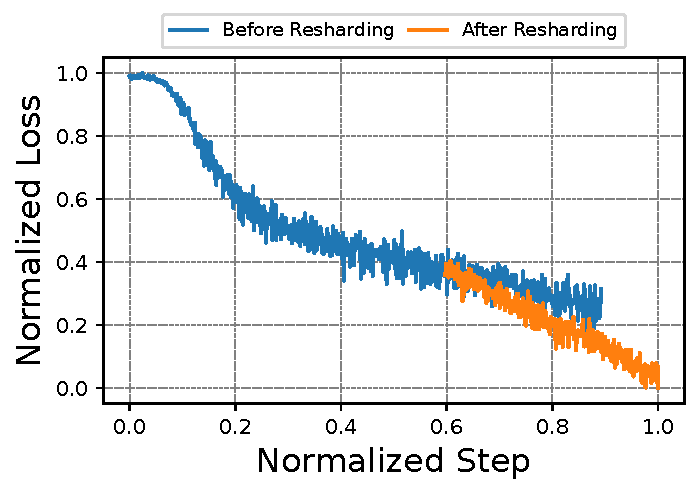
\includegraphics[width=\linewidth]{figures/dp_resharding.pdf}
         \caption{DP resharding：TP=1, DP=4, PP=4 $\rightarrow$ TP=1, DP=8, PP=4。}
         \label{fig:dp_resharding}
     \end{subfigure}
     \hfill
     \begin{subfigure}[b]{0.49\linewidth}
         \centering
         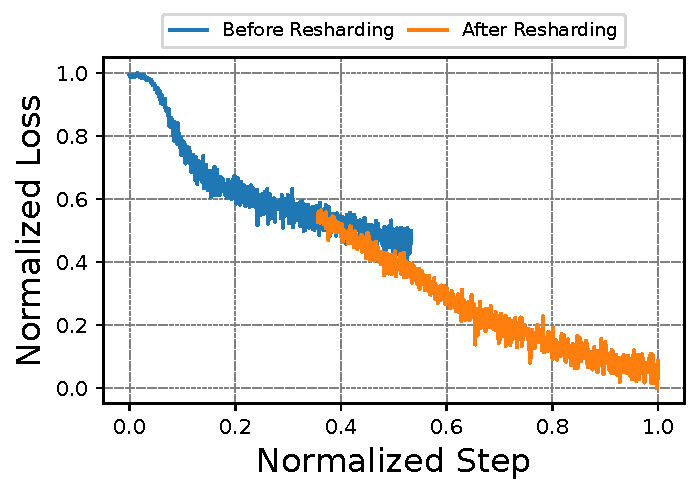
\includegraphics[width=\linewidth]{figures/hp_resharding.pdf}
         \caption{混合 resharding：TP=1, DP=4, PP=4 $\rightarrow$ TP=2, DP=8, PP=2。}
         \label{fig:hp_resharding}
     \end{subfigure}
     \caption{Resharding 正确性验证。}
      \label{fig:reshard_full_correct}
\end{figure}

\begin{figure}[!t]
  \centering
  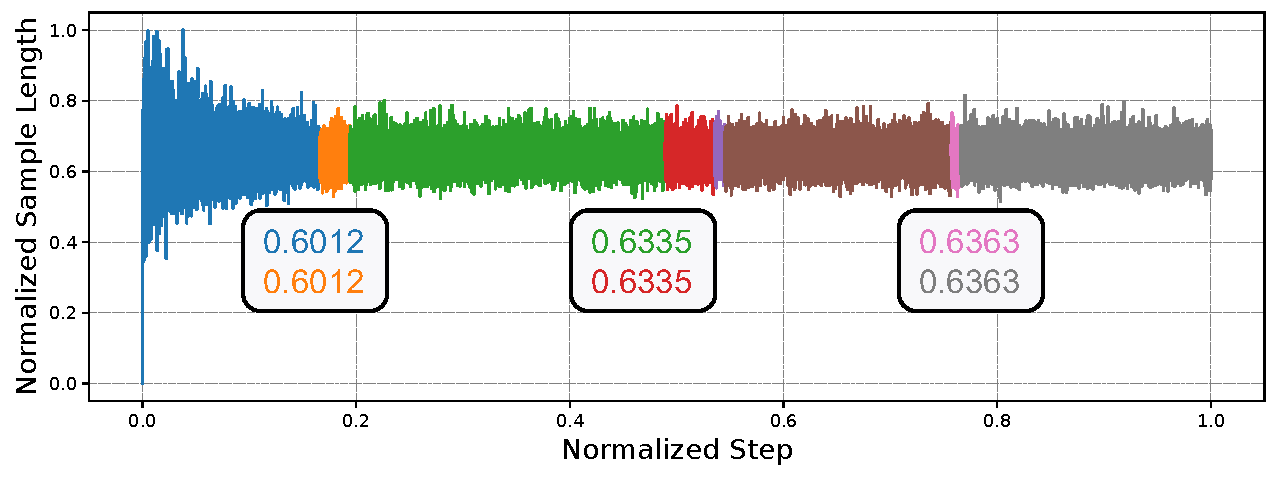
\includegraphics[width=\linewidth]{figures/online_resume_length.pdf}
  \caption{
  多次训练重启下 dataloader 的归一化样本长度曲线。
  }
  \label{fig:loader_resume}
\end{figure}


在 DP 与混合 resharding 的正确性验证中，归一化 loss 曲线如图~\ref{fig:reshard_full_correct} 所示。
由于在 DP 与混合 resharding 中我们同时增大了全局 batch size，resharding 后的 loss 下降更快。

我们进一步验证 \sys{} 可以对 dataloader 状态实现 bitwise 正确的恢复。
由于 RNG 状态固定，正确恢复应产生相同的数据采样轨迹。
因此我们使用归一化样本长度曲线（图~\ref{fig:loader_resume}）进行评估。
结果显示，重启前后的归一化样本长度曲线一致。

\section{相关工作}
\label{sec:related_work}

\noindent \textbf{Checkpointing 框架。}
一些工业实践专注于深度学习 checkpointing 系统。
在 DCP~\cite{torch-dcp} 之前，PyTorch 仅提供 \texttt{torch.save} 与 \texttt{torch.load} 用于本地 checkpoint 管理，缺乏原生 resharding 支持。
DCP~\cite{torch-dcp} 为 FSDP 引入了 resharding 能力，但不支持 TP、PP 等混合并行策略。
DeepSpeed-UCP~\cite{deepspeed-ucp} 提供统一的 DeepSpeed checkpoint 格式，并通过离线脚本实现 resharding。
Megatron MCP~\cite{megatron-dcp} 复用 DCP~\cite{torch-dcp} 的 workflow，并扩展到 Zarr~\cite{Zarr} 等存储格式。
这些框架对不同并行策略与训练框架的支持均有限，且在大规模训练中 I/O 性能与可扩展性不足。

\noindent \textbf{Checkpointing 优化。}
一些工作~\cite{projectadam, deepfreeze} 从不同角度降低 checkpointing 成本。
Check-N-Run~\cite{check-n-run} 面向推荐模型，采用差分 checkpointing 仅存储修改部分，并结合量化降低 checkpoint 大小。
CheckFreq~\cite{checkfreq} 将 snapshot 与保存与计算进行流水线化，减少 checkpoint stall，并引入在线算法调优 checkpoint 频率。
Gemini~\cite{gemini-sys} 倡导 in-memory checkpointing 与跨机器备份以加速恢复，并将 checkpoint 通信与训练流量交错，实现每次迭代的高频 checkpoint。
JIT-Checkpointing~\cite{jit-check} 采用 just-in-time checkpointing 进行低成本错误恢复。
在工业用例中，仍需将 checkpoints 保存到独立持久化存储，以支持 auto-evaluation~\cite{characterization}、超参调优与模型调试等任务。
ServerlessLLM~\cite{serverlessllm} 关注 serverless 推理场景下的加载优化，提出基于 chunk 的多级加载 pipeline 以加速 checkpoint 加载。
与这些方案不同，\sys{} 同时强调优化 I/O 性能与灵活的 load-time checkpoint resharding，面向通用 LFM 开发场景。

\noindent \textbf{Checkpoint 表示。}
PyTorch 的 \texttt{torch.save/load} 基于 \texttt{pickle} 进行序列化/反序列化，该格式缺乏全局形状等关键 shard metadata，无法支持自动 resharding。
DCP~\cite{torch-dcp} 通过将 metadata 与 tensor 数据分离来解决这一问题，metadata 包含全局形状与偏移信息，从而支持自动 resharding。
Tenplex~\cite{tenplex} 提出 Parallelizable Tensor Collection（PTC）以灵活表示与转换不同 parallelism 配置下的 tensor 状态。
\sys{} 采用 DCP 的表示并扩展以处理 irregular tensor 分片，从而构建 PyTorch-native 的 checkpointing 系统。
数组式存储系统如 Zarr~\cite{zarrZarr} 与 TensorStore~\cite{googleTensorStore} 可将 tensor 保存为独立数组，支持并发读写；MCP~\cite{megatron-dcp} 通过 Zarr 实现分布式 checkpointing。
Safetensors~\cite{huggingfaceSafetensors} 提供安全高效的 tensor 存储与加载格式。
为增强与 Hugging Face 生态兼容性，\sys{} 支持导出 Safetensors 格式的 checkpoints。

\noindent \textbf{LFM 的存储系统。}
大规模 checkpointing 需要稳健的存储系统。
LLaMA 3.1 报告~\cite{llama3.1} 指出 Tectonic~\cite{tectonic}（Meta 的通用文件系统）是 pre-training 期间存储 checkpoints 的骨干，其核心挑战之一是高频 checkpoint 写入。
类似地，DeepSeek 开发的 AI-HPC 系统 FireFlyer~\cite{fireflyer}（用于 LFM 训练~\cite{deepseekai,deepseek-v3,deepseek-r1}）采用自研 3FS 分布式文件系统~\cite{3fs}，与 BeeGFS~\cite{herold2014introduction} 等并行文件系统类似，用于 checkpoint 存储。

\noindent \textbf{弹性训练系统。}
一些正交研究致力于提升 DL 训练任务的弹性~\cite{varuna, bamboo, easyscale, parcae, swift, oobleck}。
例如，Varuna 引入 \textit{job morphing} 以在不改变超参的情况下调整 pipeline 与 data parallelism 度；
Bamboo~\cite{bamboo} 将跨阶段冗余计算融入 pipeline，以支持 spot 实例上的弹性训练；
Oobleck~\cite{oobleck} 通过预定义模板进行 pipeline 实例化，以容忍不同 pipeline 的并发故障。
这些工作通常仅覆盖特定并行策略（如不含 ZeRO 的 DP），而 \sys{} 不假设具体 parallelism，可支持真实生产场景。
采用我们的 checkpoint 表示可进一步增强弹性训练系统的状态管理能力。

